\def\handout{0}   % set to 1 to produce 4-up handouts instead of slides
\def\notes{0}     % set to 1 to show \note{}s
\def\adminstuff{0}
%%%%%%%%%%% Beamer  customization file  %%%%%%%%%%%%
%%%%%%%%%%% For giving lectures %%%%%%%%%%%%%%%%%%%%



\ifnum\handout=1  % see above for an alternative which uses two preamble files
\documentclass[handout,13pt,compress,c]{beamer}
\usepackage{algorithm,algorithmic}
\usepackage[final]{pgfpages}
\usepackage{comment}
\usepackage{handoutWithNotes}
\usepackage{pifonts}
%\setbeameroption{second mode text on second screen}
%\pgfpagesuselayout{4 on 1}[letterpaper,landscape,border shrink=4mm]
\pgfpagesuselayout{3 on 1 with notes}[letterpaper,landscape,border shrink=0.5in]

% or: \pgfpagesuselayout{2 on 1}[letterpaper,border shrink=4mm]
\setbeamertemplate{footline}[page number]   % omit if don't want slide number at bottom right
% use \setbeamertemplate{footline}[text line]{xxxx} if you want xxxx at bottom left of each slide
% use \setbeamertemplate{footline}[text line]{xxxx\hfill\thepage}
%  if you want xxxx at bottom left, page # at bottom right
\else
\documentclass[13pt,compress,c]{beamer}
\fi


%%% Themes, font, color, 
% \usetheme{CambridgeUS}
% \usetheme{PaloAlto}
% \usetheme{Berkeley}
% \usetheme{AnnArbor}
% \usetheme{Boadilla}
% \usetheme{AnnArbor}
\usetheme{CambridgeUS}
\usecolortheme{beaver}
% \usecolortheme{crane}
% \usecolortheme{wolverine}
% \usecolortheme{dolphin}
\usefonttheme[onlymath]{serif}
%\usefonttheme{serif}
%\usepackage[T1]{fontenc}
%\usepackage[scaled]{helvet}
%\usepackage{arev}
% Also try PaloAlto, Warsaw, Malmoe, Madrid, Berlin, Darmstadt; see
%  /usr/share/texmf/tex/latex/beamer/themes/theme and the above gallery.
% PaloAlto has section and subsection titles in left panel with highlighting
% Darnstadt shows section names at top with progress bubbles
% \usefonttheme{serif}
% Another nice theme courtesy of David Airey:
% \usetheme[secheader]{Boadilla}                                                                                                                                       
% \definecolor{mygold}{rgb}{0.85, 0.60, 0.00}                                                                                                                          
% \usecolortheme[named=mygold]{structure}                                                                                                                              
% \setbeamercovered{dynamic}                                                                                                                                           


\usepackage{graphicx}
\usepackage{natbib}           % for author year citations \citet \citep
\usepackage{relsize}          % for \smaller etc.
\DeclareGraphicsExtensions{.pdf, .jpg, .png}

\ifnum\notes=1 \setbeameroption{show notes} \fi
\usepackage{mydef}

%%% logos

\usepackage[absolute,overlay]{textpos}

\newcommand{\unilogo}{
  \setlength{\TPHorizModule}{1pt}
  \setlength{\TPVertModule}{1pt}
   % textblock{}{x,y}: pos(x) = leftUpperCorner + (x * \TPHorizModule), pos(y) = leftUpperCorner - (y * \TPVertModule)
  %\begin{textblock}{1}(8,245)
  % \figw{USClogoSimple2.jpg}{.123}
  %\end{textblock}
  }

%\logo{\figw{USClogoSimple2.jpg}{.123}}


\mode<presentation>
\hypersetup{pdfpagemode=FullScreen}
\AtBeginSection[]
{
   \begin{frame}
       \ft{Outline}
       \tableofcontents[currentsection,hideothersubsections]
   \end{frame}
}

\setbeamertemplate{caption}{\insertcaption}

%%%%% Mathematics %%%%
%\input{math_definition}
\usepackage{pdfpages}
\usepackage{algorithm,algorithmic}
%% COVER PAGE
% \date{September 21, 2017}
\title{Introduction to Development}
\author{Aman Agrawal}
% \institute{aman.cs115@cse.iitd.ac.in}



%\input{customize}
\date{}
\usepackage{hyperref}
\hypersetup{colorlinks,urlcolor=blue}
\usepackage{graphicx}  % remove 'demo' option for your real document

\begin{document}

\begin{frame}
\title{Introduction to Development}
\author{Aman Agrawal}
\institute{aman.cs115@cse.iitd.ernet.in}
\titlepage
\end{frame}
\section{Introduction}
    \begin{frame}{About Us}
        \uncover<+->{Here is what our website says:\\}
        \uncover<+->{
        \begin{quote}
            Dev Club is a student group that tries to innovate and foster technical activities, and create a coding culture which is somewhat missing.             
        \end{quote}
        }
    \end{frame}
    \begin{frame}{Missing??}
        \uncover<+->{
        \begin{itemize}
            \item<+-> Non Existent
            \item<+->[] Have you seen anyone around you developing anything interesting?
            \item<+-> No One Cares
            \item<+->[] No one questions the fact that our college is not as \textbf{''technical''} as it should be.
            \item<+-> No initiative
            \item<+->[] Lack of any community of interested people (unlike cultural case)   
        \end{itemize}
        }
    \end{frame}
    \begin{frame}{Is it same in other IITs??}
        \uncover<+-> {\textbf {Ofcourse Not!!\\}}
        \uncover<+->{Like:\\}
        \begin{itemize}
            \item<+-> \href{https://sdslabs.co}{SDS Labs} : IIT Roorkee
            \item<+-> \href{http://pclub.in/}{Programming Club} : IIT Kanpur            
            \item<+-> \href{http://wncc-iitb.org}{Web and Coding Club} :  IIT Bombay
            \item<+-> \href{http://kossiitkgp.in/}{Kharagpur Open Source Society} :  IIT KGP
            \item<+->[] \textbf{And Now !!}
            \item<+-> \href{http://www.cse.iitd.ernet.in/devclub/}{Dev Club} : IIT Delhi
        \end{itemize}
    \end{frame}
\section{Software Development}
    \begin{frame}{What is Software Development?}
        \uncover<+->{Here is what wikipedia says:\\}
        \uncover<+->{
        \begin{quote}
            Software development is the process of computer programming, documenting, testing, and bug fixing involved in creating and maintaining applications and frameworks resulting in a software product.
        \end{quote}
        }
        
    \end{frame}
    \begin{frame}{Why is it useful?}
        \begin{itemize}
            \item<+-> You will become a better, more efficient, and less error-prone coder.
            \item<+-> Necessary for a lot of coding jobs and something that is NOT taught in college            
            \item<+-> Meet other motivated and like minded smart students.
        \end{itemize}
    \end{frame}
    \begin{frame}{Perks!!}
        \uncover<+->{Get Selected for competitions like \textbf{GSOC}\uncover<+->{  and get sipend of \textit{1.5 Lakhs}}\\}
        \vspace{20px}
        \uncover<+->{Win in \textbf{Microsoft Code.fun.do} \uncover<+->{ and win an all expenses paid trip!!}\\}
        \vspace{20px}        
        \uncover<+->{Be the \textbf{CTO} and \textbf{CEO} of your own startup!!}
        
    \end{frame}
    \begin{frame}{Pre-requisites}
        Here are some pre requisites:
        \pause
        \begin{itemize}
            \item<+-> Language basic of either C++, Java or Python.
            \item<+-> Ability to read documentations effeciently.
            \item<+-> Able to do a good GOOGLE Search !!            
            \item<+->[] \textit{And most importantly,}
            \item<+-> Perseverance
        \end{itemize}
    \end{frame}
    \begin{frame}{What Can we learn?}
        \begin{itemize}
            \item<+-> Making \textbf{best UI/UX} using angular, react, bootstrap, etc.
            \item<+-> \textbf{Server side management} : Docker, Resource management, Sandboxing, Monitoring, etc.
            \item<+-> \textbf{Back end} : Node.js, Django, Rust, Scala, Julia....
            \item<+-> \textbf{Tools} : Git, Slack, IRC, Database (SQL, NoSQL ..)..
            \item<+-> And a hell lot which even we don’t know that we don’t know
        \end{itemize}
    \end{frame}

\section{About Us}
    \begin{frame}{Our Work}
        \uncover<+->{We develop cool stuff that benefits everyone in the campus.\\}
        \uncover<+->{Like:\\}
        \begin{itemize}
            \item<+-> \href{https://aman71197.github.io/CampusBot/}{Campus Bot}
            \item<+-> \href{http://iitd.info/study_portal}{Study Portal}            
            \item<+-> \href{http://10.17.51.99:3000/}{Multiplayer Game}
            \item<+-> \href{http://sendata.herokuapp.com/}{SenData}
            \item<+-> \href{http://www.cse.iitd.ernet.in/devclub/}{Our own Website}
        \end{itemize}
    \end{frame}
    \begin{frame}{Our Aim}
        \uncover<+->{Short Term\\}
        \begin{itemize}
            \item<+-> Develop a community of like minded people !
            \item<+-> Revive, maintain and popularise applied computer science aspects.            
            \item<+-> Take up all the software development work happening in the campus, like academics website, RDV, Tryst etc.
        \end{itemize}
        \uncover<+->{Long Term\\}
    \uncover<+->{\begin{center} \textbf{Go Commercial !!} \end{center}}
    \end{frame}
\section{Getting Started}
    \begin{frame}{Learn about}
        \begin{columns}
            \column{.5\textwidth}
            \begin{itemize}
                \onslide<1->{\item Git : Make a student account}
                \onslide<2->{\item Linux Bash}            
                \onslide<3->{\item Start Developing something}
            \end{itemize}
            \column{.5\textwidth}
            \begin{figure}
                \onslide<1->{
\includegraphics[width=1\linewidth]{imgs/git.png}\\}
                \onslide<2->{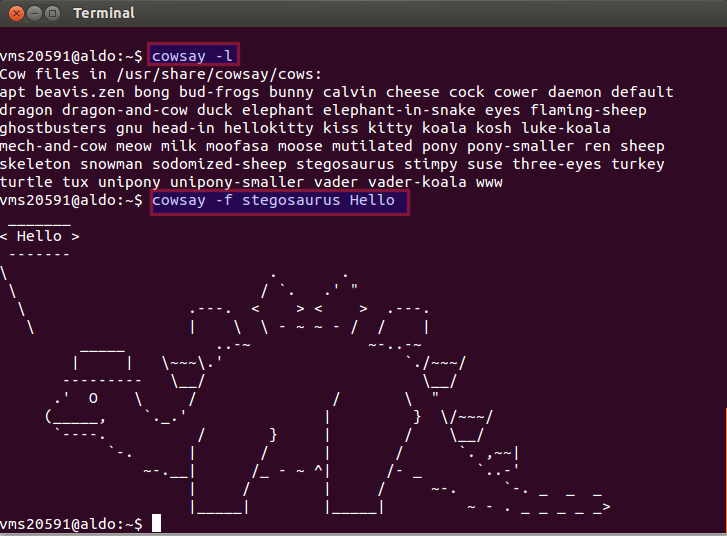
\includegraphics[width=1\linewidth]{imgs/cmd.png}}
            \end{figure}
        \end{columns}
    \end{frame}
    \begin{frame}{Real Friends:}
    \begin{columns}
        \column{.5\textwidth}
        Google and Stackoverflow :)
        \column{.5\textwidth}
        \begin{figure}
        
\includegraphics[width=1\textwidth]{imgs/friends.jpg}
        \end{figure}
        \end{columns}
    \end{frame}
    \begin{frame}{Lectures}
        \uncover<+-> { Attend Lectures that will be held soon}    
    \end{frame}
\section{Getting Involved}
    \begin{frame}{Github Org}
        \begin{itemize}
            \item<+-> Look at our github repo and ongoing projects : \uncover<+->{\href{https://github.com/devclub-iitd}{Repo}}
            \item<+-> Select a project which interests you
            \item<+-> Look at the TODO list and Bugs needed to be fixed
            \item<+-> Develop the functionality or fix Bugs
            \item<+-> Generate a pull request
        \end{itemize}
    \end{frame}
    \begin{frame}{Recruitment}
        \uncover<+-> {We will have a official recruitment process, next semester in January\\ }
        \vspace{20px}
        \begin{center}
        \uncover<+-> { Till then Happy Developing !!}  
        \end{center}      
    \end{frame}

\end{document}

